\documentclass[10pt]{article}

% Specify the margins and text size.
\setlength{\textwidth}{6.4in}
\setlength{\textheight}{9.5in}
\setlength{\oddsidemargin}{0pt}
\setlength{\evensidemargin}{0pt}
\setlength{\topmargin}{0pt}
\setlength{\hoffset}{.05in}
\setlength{\voffset}{-1in}

\setlength{\parskip}{5pt}
\setlength{\parindent}{0pt}

% Load some fonts and symbol packages
\usepackage{latexsym}
\usepackage{pifont}       % contains 'star' symbol for counterinsurgency handbook title
\usepackage{yfonts} 
\usepackage{amsmath}
\usepackage{amsfonts}

\usepackage{graphicx}     % actually, this is loaded by pstricks
\usepackage[T1]{fontenc}
\usepackage{ifthen}
\usepackage{pstricks,pst-grad,pst-text,pst-node,multido,pst-plot,calc,pst-3dplot}
%\usepackage[all]{xy}
%\usepackage{animate}

% The hyperref package inserts links into the pdf.
\definecolor{MyLinkColor}{rgb}{.1,.2,1}
\definecolor{MyCiteColor}{rgb}{.1,1,.2}
\definecolor{MyURLColor}{rgb}{.4,.4,.4}
\usepackage[backref=true,pagebackref=false,hyperindex,colorlinks=true,
  linkcolor=MyLinkColor,urlcolor=MyURLColor]{hyperref}


% The tweaklist package is something I found on the web.  It provides a simple interface
% for making changes to spacing used in the itemize and enumerate environments.  Comment
% this out if you don't care to use tweaklist.
\usepackage{tweaklist}
\renewcommand{\itemhook}{\setlength{\parskip}{2pt}\setlength{\parsep}%
{1pt}\setlength{\topsep}{0pt}\setlength{\itemsep}{0pt}}

\newcommand{\U}{\underline{\hspace{5pt}}}

\usepackage{listings}
\newcommand{\Z}{\hphantom{0}}

\begin{document}
\pagestyle{empty}
\lstset{language=R, showspaces=false, showstringspaces=false}

\href{http://www.su.edu}{
\includegraphics[height=1.75cm]{sulogo.eps}}
\vspace{-1.69cm}

{{\ }\hfill\small
\begin{tabular}{cl}
& Math 207\\
& Introduction to Statistics\\
\end{tabular}
}
\setlength{\baselineskip}{1.05\baselineskip}

\begin{center}
\textbf{\large  Quiz: Regression}
\end{center}
\medskip

1. The length of odontoblasts (tooth cells) in each of 10 guinea pigs 
at each of three dose levels of vitamin~C (0.5, 1, and 2 mg) 
is measured.  The scatter plot of the data is shown below.

\begin{center}
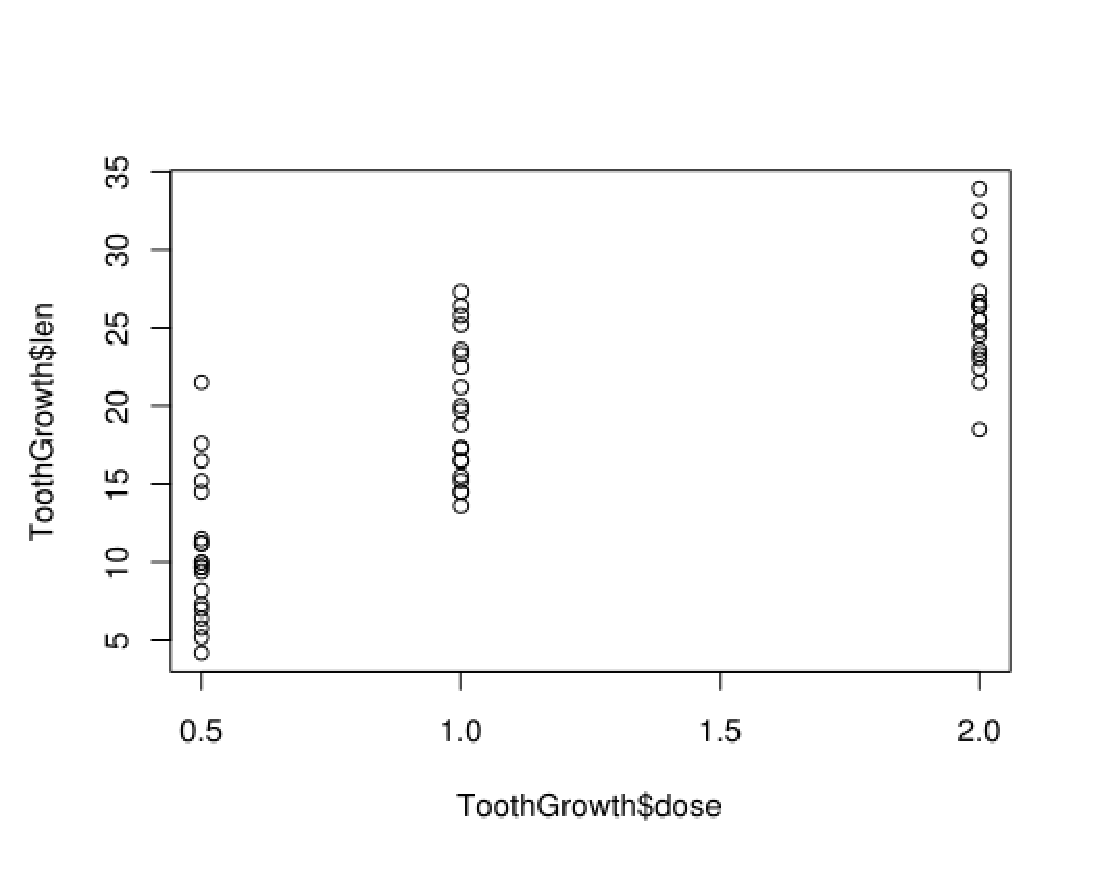
\includegraphics[height=1.75in,bb=0 22 515 340, clip]{teeth.eps}
\end{center}
The equation for the regression line computed from the data is 
\[y \approx 10\,x + 7\]
where $x$ is dose level in mg and $y$ is odontoblast length.
The correlation coefficient for the data is $r\approx 0.8$.

\hspace{20pt} a) Sketch the regression line in the above plot.

{\color{blue}The line contains these points:\vspace{-15pt}
\begin{center}
\begin{tabular}{ccccc}
$x$ & 0.5 & 1.0 & 1.5 & 2.0\\
$y$ & 12 & 17 & 22 & 27
\end{tabular}
\end{center}}

\hspace{20pt} b) Estimate the odontoblast length if the dose level is $1.5$ mg.

{\color{blue}  If $x=1.5$, then $y=22$ is the estimate (the point on the line).}
\bigskip

\hspace{20pt} c) The RMS error for the regression line is $4.5$.
Among guinea pigs that receive a vitamin C dose level of 2 mg, 68\% 
  have odontoblast length in what range?

{\color{blue} If $x=2$, then $y=27$ is the prediction.  Since we want 
a range for 68\% of the points (with $x=2$), we 
use \[27\pm 1\times \mbox{RMS}=27\pm 4.5.\]}

  \hspace{20pt} d) 
Among guinea pigs that receive a vitamin C dose level of 1.5 mg, 95\% 
  have odontoblast length in what range?

{\color{blue} If $x=1.5$, then $y=22$. Since we want a range for
95\% of the points (with $x=1.5$), we 
use \[22\pm 2\times \mbox{RMS}=27\pm 4.5 = 22\pm 9.\]}

\hspace{20pt} e) One measurement has $\mbox{dose}=1.0$ mg and 
$\mbox{length}=14.0$. Calculate the length predicted by the regression
line then calculate the  residual error for that value: $y - (\mbox{predicted value})$.

{\color{blue} The predicted value is 17 if $x=1$.  So, the error is 
$14-17 = -3$.  }
\vfill
\eject

2. For men age 25--34, the relationship between education (years of schooling
completed) and systolic blood pressure can be summarized as follows.
\begin{align*}
\mbox{average education} &\approx 13 \mbox{ years},
  & \mbox{sd} &\approx 3 \mbox{ years}\\
\mbox{average blood pressure} &\approx 119 \mbox{ mm}
  & \mbox{sd} &\approx 12 \mbox{ mm}
\end{align*}
The correlation coefficient is $r\approx -0.1$.

\hspace{20pt} a) Sketch the regression line and write down its equation.

{\color{blue} The equation is\vspace{-15pt}
\begin{align*}
y - 119 &= -0.1\,\frac{12}{3}\,(x-13)\\
y - 119 &= -0.4\,(x-13)
\end{align*}
This is a line that contains the point $(13, 119)$ and has slope $-0.4$.}
\bigskip

\hspace{20pt} b) Predict the blood pressure of a man with 20 years of education.

{\color{blue}
If $x=20$, then $y=119 - 0.4\,(20 - 13) = 119 - 0.4\times 7 = 119-2.8 = 16.2$.
Our prediction is the point on the line.}
\medskip

\hspace{20pt} c) Estimate the average blood pressure among all subjects with 20 years of education.

{\color{blue} Numerically, our answer is 16.2 again.  The reason is that
the \textit{average} of the $y$-values for dots with $x=20$ \underline{is}
the point on the line (which we calculated in b).}
\bigskip

\hspace{20pt} d) One subject  had 20 years of education, and his 
blood pressure was 118~mm.  True or false and explain:  compared to other men
at his educational level, his blood pressure was a bit on the high side.

{\color{blue} His $z$ score is $z=(118 - 116.2)/\mbox{RMS}$ since 
RMS is standard deviations for the normal curves that move along 
the regression line.  The value is:
\[\mbox{RMS}=\mbox{sd}_y\,\sqrt{1-r^2} = 12\,\sqrt{1 - (-0.1)^2} \approx 12.\]
So, the subject's $z$ score is $z\approx (118-116.2)/12=1.8/12 = 0.15$.
That is close to the center of the normal curve.  So, his blood 
pressure is about average.}
\bigskip

\hspace{20pt} e) Suggest reasons for the sign ($\pm 1$) and magnitude ($0.1$) of $r$.

{\color{blue} The correlation is negative.  That means subjects with
more education had lower blood pressure.  Perhaps that is because
they have better jobs and, consequently, better health care.  

The correlation is close to zero, however.  That means education
level is not a good predictor of blood pressure.  Diet and exercise
would have much stronger correlations.}

\vfill
\eject          

\end{document}

